%% This file explains the options available to you for editing the file
%% main.tex.

%% The commands in this file allow you to specify options such as
%% spacing, double-sided printing, a draft copy, etc.   By default, 12pt
%% and lgrind are included; lgrind is the 2e style for including code in
%% your thesis.

%% \documentclass[12pt]{mitthesis}
%% \usepackage{lgrind}
%% \pagestyle{plain}

%% You can add options in the documentclass line as follows:

%% 	o  singlespace
%% 	\documentclass[12pt,singlespace]{mitthesis}
	
%% 	o  twoside
%% 	\documentclass[12pt,twoside]{mitthesis}

%% 	o  draft   (make sure to change the pagestyle to drafthead as well)
%% 	\documentclass[12pt,draft]{mitthesis}
%% 	\usepackage{lgrind}
%% 	\pagestyle{drafthead}

%% 	o vi   (for course vi and course viii theses)
%% 	\documentclass[12pt,vi]{mitthesis}

%% Any options you would use for report.sty will work here as well.


%% You should not need to change the first three lines and last two lines
%% below.  Be sure to include an \include command for each file you are
%% including in your thesis.
  
%% % -*-latex-*-
% 
% For questions, comments, concerns or complaints:
% thesis@mit.edu
% 
%
% $Log: cover.tex,v $
% Revision 1.9  2019/08/06 14:18:15  cmalin
% Replaced sample content with non-specific text.
%
% Revision 1.8  2008/05/13 15:02:15  jdreed
% Degree month is June, not May.  Added note about prevdegrees.
% Arthur Smith's title updated
%
% Revision 1.7  2001/02/08 18:53:16  boojum
% changed some \newpages to \cleardoublepages
%
% Revision 1.6  1999/10/21 14:49:31  boojum
% changed comment referring to documentstyle
%
% Revision 1.5  1999/10/21 14:39:04  boojum
% *** empty log message ***
%
% Revision 1.4  1997/04/18  17:54:10  othomas
% added page numbers on abstract and cover, and made 1 abstract
% page the default rather than 2.  (anne hunter tells me this
% is the new institute standard.)
%
% Revision 1.4  1997/04/18  17:54:10  othomas
% added page numbers on abstract and cover, and made 1 abstract
% page the default rather than 2.  (anne hunter tells me this
% is the new institute standard.)
%
% Revision 1.3  93/05/17  17:06:29  starflt
% Added acknowledgements section (suggested by tompalka)
% 
% Revision 1.2  92/04/22  13:13:13  epeisach
% Fixes for 1991 course 6 requirements
% Phrase "and to grant others the right to do so" has been added to 
% permission clause
% Second copy of abstract is not counted as separate pages so numbering works
% out
% 
% Revision 1.1  92/04/22  13:08:20  epeisach

% NOTE:
% These templates make an effort to conform to the MIT Thesis specifications,
% however the specifications can change. We recommend that you verify the
% layout of your title page with your thesis advisor and/or the MIT 
% Libraries before printing your final copy.

\title{Fault-Tolerant All-Pairs Mincuts}

\author{Abhyuday Pandey\\(BT/CSE/170039)\\\\\\\textbf{Supervisor:} Dr. Surender Baswana}
\date{\today}

% \maketitle
% \begin{center}
%     
\includegraphics[]{templates/iitk_logo.jpg}
% \end{center}

\makeatletter
    \begin{titlepage}
        \begin{center}
            {\huge \bfseries  \@title }\\[4ex] 
            {\large  Abhyuday Pandey}\\[4ex]
            {\large BT/CSE/170039}\\[4ex]
            {\large \textbf{Supervisor:} Dr. Surender Baswana}\\[20ex]
            
\includegraphics[height=5cm]{templates/iitk_logo.jpg}\\[20ex] 
            
            {\large \@date}
        \end{center}
    \end{titlepage}
\makeatother
\thispagestyle{empty}
\newpage

% The abstractpage environment sets up everything on the page except
% the text itself.  The title and other header material are put at the
% top of the page, and the supervisors are listed at the bottom.  A
% new page is begun both before and after.  Of course, an abstract may
% be more than one page itself.  If you need more control over the
% format of the page, you can use the abstract environment, which puts
% the word "Abstract" at the beginning and single spaces its text.

%% You can either \input (*not* \include) your abstract file, or you can put
%% the text of the abstract directly between the \begin{abstractpage} and
%% \end{abstractpage} commands.

% First copy: start a new page, and save the page number.
% Uncomment the next line if you do NOT want a page number on your
% abstract and acknowledgments pages.
% \pagestyle{empty}
\section*{Abstract}
\subfile{abstract}
\vfill
% {These results are submitted to the $53^{rd}$ Annual ACM Symposium on Theory of Computing
% June $21-25, 2021$ in Rome, Italy.}

\pagebreak
% Additional copy: start a new page, and reset the page number.  This way,
% the second copy of the abstract is not counted as separate pages.
% Uncomment the next 6 lines if you need two copies of the abstract
% page.
% \setcounter{page}{\thesavepage}
% \begin{abstractpage}
% % $Log: abstract.tex,v $
% Revision 1.1  93/05/14  14:56:25  starflt
% Initial revision
% 
% Revision 1.1  90/05/04  10:41:01  lwvanels
% Initial revision
% 
%
%% The text of your abstract and nothing else (other than comments) goes here.
%% It will be single-spaced and the rest of the text that is supposed to go on
%% the abstract page will be generated by the abstractpage environment.  This
%% file should be \input (not \include 'd) from cover.tex.

Let $G=(V,E)$ be an undirected unweighted graph on $n$ vertices and $m$ edges. We address the problem of sensitivity oracle for all-pairs mincuts in $G$ defined as follows.

Build a compact data structure that, on receiving a pair of vertices $s,t\in V$ and insertion/deletion of any edge as query, can efficiently report the value of the mincut between $s$ and $t$ upon the update.

To the best of our knowledge, there exists no data structure for this problem which takes $o(mn)$ space and a non-trivial query time. Recently, Baswana, Gupta, and Knollman \cite{DBLP:conf/esa/BaswanaGK20} gave a data structure that can handle single edge insertion in ${\cal O}(n^2)$ space and ${\cal O}(1)$ query time. We present the following results.

\begin{enumerate}
    \item We present a sensitivity oracle for all-pairs mincuts. Our data structure guarantees ${\cal O}(1)$ query time. The space occupied by this data structure is ${\cal O}(n^2)$ which matches the worst-case size of a graph on $n$ vertices. A resulting $(s,t)$-mincut after edge insertion/deletion can be reported in ${\cal O}(n)$ time which is optimal. Our data structure also subsumes the results of Baswana, Gupta, and Knollman \cite{DBLP:conf/esa/BaswanaGK20}.
    \item We give conditional lower bounds on data structures that can handle dual-deletions (or dual-faults) for a $(s,t)$-mincut. We also give a conditional lower bound on a data structure storing all static $(\{s,u\},\{t,v\})$-mincut values with fixed $s,t \in V$. This implies a conditional lower bound for a generalized flow tree for $2 \times 2$ mincuts, i.e. a data structure that can report the value of static $(\{s,u\},\{t,v\})$-mincut for given vertices $s,t,u,v \in V$.
\end{enumerate}

Some parts of this work have been taken from a recent research of Baswana and Pandey \cite{DBLP:journals/corr/BaswanaP20}, but presented here for sake of continuity. 

% \end{abstractpage}

\section*{Acknowledgments}

I am deeply indebted to Prof Surender Baswana for allowing me to work with him. I am thankful to him for having regular meetings despite his busy schedule and helping me acquire the necessary perseverance for solving a research problem. I would like to thank Prof Yefim Dinitz and Prof Alek Vainshtein for their seminal work ``The connectivity carcass of a vertex subset in a graph and its incremental maintenance" which appeared in STOC 1994 and subsequently in SIAM Journal of Computing 2000 edition. The paper truly captures the entire anatomy of mincuts and also forms the foundation of our results. Last but not the least, I would like to thank my parents and sister for their incredible and unconditional support in this pandemic. 
%%%%%%%%%%%%%%%%%%%%%%%%%%%%%%%%%%%%%%%%%%%%%%%%%%%%%%%%%%%%%%%%%%%%%%
% -*-latex-*-

%% \pagestyle{plain}
%%   % -*- Mode:TeX -*-
%% This file simply contains the commands that actually generate the table of
%% contents and lists of figures and tables.  You can omit any or all of
%% these files by simply taking out the appropriate command.  For more
%% information on these files, see appendix C.3.3 of the LaTeX manual. 
\tableofcontents
% \newpage
% \listoffigures
% \newpage
% \listoftables


%% %% This is an example first chapter.  You should put chapter/appendix that you
%% write into a separate file, and add a line \include{yourfilename} to
%% main.tex, where `yourfilename.tex' is the name of the chapter/appendix file.
%% You can process specific files by typing their names in at the 
%% \files=
%% prompt when you run the file main.tex through LaTeX.
\chapter{Introduction}

Graph mincut is a fundamental structure in graph theory with numerous applications. Let $G=(V,E)$ be an undirected unweighted connected graph on $n=|V|$ vertices and $m=|E|$ edges.
Two most common types of mincuts are global mincuts and pairwise mincuts. A set of edges with the least cardinality whose removal disconnects the graph is called a global mincut. For any pair of vertices $s,t\in V$, 
a set of edges with the least cardinality whose removal disconnects $t$ from $s$ is called a pairwise mincut for $s,t$ or simply a $(s,t)$-mincut. A more general notion is that of Steiner mincuts. For any given set $S\subseteq V$ of vertices, a set of edges with the least cardinality whose removal disconnects $S$ is called a Steiner mincut for $S$. It is easy to observe that the Steiner mincuts for $S=V$ are the global mincuts and for $S=\{s,t\}$ are $(s,t)$-mincuts.

While designing an algorithm for a graph problem, one usually assumes that the underlying graph is static. But, this assumption is unrealistic for most of the real-world graphs where vertices and/or edges do undergo change, though occasionally. Sensitivity Oracles can be used to efficiently make a query for a single update/delete operation. The data structure can be preprocessed offline.

% In the past, many elegant fault-tolerant algorithms have been designed for various classical problems, namely,  connectivity \cite{DBLP:conf/stoc/Chan02,DBLP:journals/algorithmica/FrigioniI00,DBLP:journals/siamcomp/ChanPR11,DBLP:conf/soda/DuanP17}, shortest-paths \cite{DBLP:conf/stoc/BernsteinK09,DBLP:journals/siamcomp/DemetrescuTCR08,DBLP:conf/stoc/ChechikC20}, graph spanners \cite{ChechikLPR10,DBLP:journals/tcs/BraunschvigCPS15}, SCC \cite{DBLP:journals/algorithmica/BaswanaCR19} , DFS tree \cite{DBLP:journals/siamcomp/BaswanaCC019}, and BFS structure \cite{DBLP:journals/talg/ParterP16,DBLP:journals/talg/ParterP18}. However, little is known about fault-tolerant data structures for various types of mincuts. The problem of fault-tolerant all-pairs mincuts aims at preprocessing a given graph to build a compact data structure so that the following query can be answered efficiently for any $s,t\in V$ and $(x,y)\in E$.\\

% \noindent
% FT-mincut$(u,v,x,y)$: Report the value of $(u,v)$-mincut in $G$ after the failure/removal of edge $(x,y)$, if exists, from $E$.\\

% \noindent
% % {\textsc{ft-mincut}}$(s,t,x,y)$: Report a $(s,t)$-mincut in $G$ after the failure of edge $(x,y)$, if exists, from $E$.\\
% {\textsc{ft-mincut}}$(s,t,x,y)$: Report a $(s,t)$-mincut in $G$ after the failure of edge $(x,y)$.\\



\section{Previous Results} 


There exists a classical ${\cal O}(n)$ size data structure that stores all-pairs mincuts \cite{GH61} known as Gomory-Hu tree. It is a tree on the vertex set $V$ that compactly stores a mincut between each pair of vertices. However, we cannot determine using a Gomory-Hu tree whether the failure of an edge will affect the $(s,t)$-mincut unless this edge belongs to the $(s,t)$-mincut present in the tree. We can get a fault-tolerant data structure by storing $m$ Gomory-Hu trees, one for each edge failure. The overall data structure occupies ${\cal O}(mn)$ space and takes ${\cal O}(1)$ time to report the value of $(s,t)$-mincut for any $s,t\in V$ upon failure of a given edge. A new $(s,t)$-mincut can itself be reported in ${\cal O}(n)$ time. 


For handling edge insertions, Baswana, Gupta and Knollman \cite{DBLP:conf/esa/BaswanaGK20} recently gave a data structure that can report the value of a $(s,t)$-mincut upon insertion of an edge. Moreover, a $(s,t)$-mincut incorporating the change can be reported in ${\cal O}(n)$ time.


Combining the above two results, a sensitivity oracle can be obtained that uses ${\cal O}(mn)$ space. However, the ${\cal O}(mn)$ space occupied by this data structure is far from the size of the graph. To the best of our knowledge, there exists no data structure for this problem which takes $o(mn)$ space and a non-trivial query time.



\section{Our Contribution} We present a space efficient sensitivity oracle for the all-pairs mincuts problem in an undirected unweighted multigraph. The data structure occupies ${\cal O}(n^2)$ space while achieving the optimal ${\cal O}(1)$ query time to report the value of $(s,t)$-mincut for any $s,t\in V$ upon deletion/insertion of any given edge. A resulting $(s,t)$-mincut incorporating the change can be reported in ${\cal O}(n)$ time.

In order to design our data structure, we present an efficient solution for a related problem of independent interest, called edge-containment query on a mincut defined as follows.\\

\noindent
{\textsc{edge-contained}}$(s,t,(x,y))$: Check if a given edge $(x,y)\in E$ belong to some $(s,t)$-mincut.\\

Using a data structure for this problem, we can answer a deletion query upon failure of edge $(x,y)$ by performing the corresponding edge-containment query. The value of $(s,t)$-mincut will reduce by unity if the edge-containment query evaluates to true. We can keep a Gomory-Hu tree of ${\cal O}(n)$ size as an auxiliary data structure to lookup the old value of $c_{s,t}$. The following fact allows us to do so.

\begin{fact}
\label{fact:(x,y)-lies-in-(s,t)-mincut}
The value of $(s,t)$-mincut decreases on deletion of an edge $(x,y)$ if and only if $(x,y)$ lies in \textit{some} $(s,t)$-mincut.
\end{fact}


We give conditional lower bounds for the following problems.

\begin{enumerate}
    \item Data structures that can handle dual-deletions (or dual-faults) for a $(s,t)$-mincut. In particular, we show that a data structure that can handle deletion (or failure) of two edges for a $(s,t)$-mincut even for fixed pair of vertices $s,t\in V$ requires ${\tilde \Omega}(n^2)$ space for non-trivial query time.
    \item Generalized flow tree for $2 \times 2$ mincuts, i.e. a data structure that can report the value of static $(\{s,u\},\{v,t\})$-mincut for given vertices $s,t,u,v \in V$. We show that even if we fix $s,t \in V$, the data structure must require ${\tilde \Omega}(n^2)$ space for non-trivial query time.
\end{enumerate}


\section{Related Work} 
A related problem is that of maintaining mincuts in a dynamic environment. Until recently, most of the work on this problem has been limited to global mincuts. Thorup \cite{DBLP:journals/combinatorica/Thorup07} gave a Monte-Carlo algorithm for maintaining a global mincut of polylogarithmic size with ${\tilde {\cal O}}(\sqrt{n})$ update time.  He also showed how to maintain a global mincut of arbitrary size with $1+o(1)$-approximation within the same time-bound. Goranci, Henzinger and Thorup \cite{DBLP:journals/talg/GoranciHT18} gave a deterministic incremental algorithm for maintaining a global mincut with amortized ${\tilde{\cal O}}(1)$ update time and ${\cal O}(1)$ query time. Hartmann and Wagner \cite{DBLP:conf/isaac/HartmannW12} designed a fully dynamic algorithm for maintaining all-pairs mincuts  which provided significant speedup in many real-world graphs, however, its worst-case asymptotic time complexity is not better than the best static algorithm for an all-pairs mincut tree. Recently, there is a fully-dynamic algorithm \cite{DBLP:journals/corr/abs-2005-02368} that approximates all-pairs mincuts up to a nearly logarithmic factor in ${\tilde{\cal O}}(n^{2/3} )$ amortized time against an oblivious adversary, and ${\tilde{\cal O}}(m^{3/4} )$ time against an adaptive adversary. To the best of our knowledge, there exists no non-trivial dynamic algorithm for all-pairs \textit{exact} mincut. We feel that our insights in this paper may be helpful in this problem.

\noindent


% \section{Overview of our results} 

% Dinitz and Vainshtein \cite{DBLP:journals/siamcomp/DinitzV00}
% presented a novel data structure called {\em connectivity carcass} that stores all Steiner mincuts for a given Steiner set $S\subseteq V$ in ${\cal O}(\min(m,nc_S))$ space, where $c_S$ is the value of Steiner mincut. %We observe that this data structure can be used easily to design a fault-tolerant data structure for all-pairs mincuts that occupies $O(mn)$-space. 
% Katz, Katz, Korman and Peleg \cite{DBLP:journals/siamcomp/KatzKKP04} presented a data structure of ${\cal O}(n)$ size for labeling scheme of all-pairs mincuts. This structure hierarchically partitions the vertices based on their connectivity in the form of a rooted tree. In this tree, each leaf node is a vertex in set $V$ and each internal node $\nu$ stores the Steiner mincut value of the set $S(\nu)$ of leaf nodes in the subtree rooted at $\nu$. %stores all-pairs mincut value.
% % Apparently, both these data structures seem to be designed for a static graph. 
% We observe that if each internal node $\nu$ of the hierarchy tree
% is augmented with the connectivity carcass of $S(\nu)$, we get a data structure for the edge-containment query. This data structure occupies ${\cal O}(mn)$ space. An edge-containment query can be answered using the connectivity carcass at the Lowest Common Ancestor (LCA) of the given pair of vertices.
% %following, more generic, fault-tolerant query :

% As we move down the hierarchy tree, the size of Steiner set associated with the internal node reduces. So, to make the data structure more compact, a possible approach is to associate a smaller graph $G_\nu$ for each internal node $\nu$ that is {\em small enough} to improve the overall space-bound, yet {\em large enough} to retain the internal connectivity of set $S(\nu)$. 
% However, such a compact graph cannot directly answer the edge-containment query as it does not even contain the information about all edges in $G$. A possible way to overcome this challenge is to transform any edge-containment query in graph $G$ to an equivalent query in graph $G_{\nu}$. In this paper, we show that not only such a transformation exists, but it can also be computed efficiently. We model the query transformation as a multi-step procedure. The following result captures a single step of this procedure.

% % The key observation that allows us to do query transformation is as follows. 
% Given an undirected graph $G=(V,E)$ and a Steiner set $S\subseteq V$, let $S'\subset S$ be any maximal set with connectivity strictly greater than that of $S$. We can build a quotient graph $G_{S'}=(V_{S'},E_{S'})$ such that $S' \subset V_{S'}$ with the following property.

% {\em
% For any two vertices $s,t \in S'$ and any set of edges $E_y$ incident on vertex $y$ in $G$, there exists a set of edges $E_{y'}$ incident on a vertex $y'$ in $G_{S'}$ such that $E_y$ lies in a $(s,t)$-mincut in $G$ if and only if $E_{y'}$ lies in a $(s,t)$-mincut in $G_{S'}$. 
% }

% We build graph $G_\mu$ associated with each internal node $\mu$ of the hierarchy tree as follows. For the root node $r$, $G_r = G$. For any other internal node $\mu$, we use the above result to build the graph $G_{\mu}$ from $G_{\mu'}$, where $\mu'$ is the parent of $\mu$. 
% Our data-structure is the hierarchy tree where each internal node $\mu$ is augmented with the connectivity carcass for $G_\mu$ and the Steiner set $S(\mu)$. A high-level description of our query algorithm is as follows. 
% % We move from the root node to the LCA of $s$ and $t$.
% We traverse the path from the root node to the LCA of $s$ and $t$.
% % We keep transforming an edge-containment query for each edge in this path. 
% We keep transforming the edge-containment query for each edge in this path.
% At the LCA of $s$ and $t$, we stop and perform the query using the connectivity carcass 
% % augmented at this node
% stored at this node.
% Following a rigorous analysis, we show that this data structure takes only ${\cal O}(m)$ space and can answer any edge-containment query in ${\cal O}(\min(m,nc_{s,t}))$ time.

% \section{Organization of the paper:}

% In addition to the basic notations, Section \ref{sec:prelimiaries} presents compact representation for various mincuts. Section \ref{sec:query-transformation} gives insights into $3$-vertex mincuts that form the foundation for transforming an edge-containment query in original graph to a compact graph. We give the construction of compact graph for query transformation in Section \ref{sec:compact-graph-section}.
% Using this compact graph as a building block, we present the data structures for edge-containment query in Section \ref{sec:final-ds}.
%% \chapter{Preliminaries}


%\subsection{Notations and lemmas on mincuts}
Let $G=(V,E)$ be an undirected unweighted multigraph without self-loops. To contract (or compress) a set of vertices $U\subseteq V$ means to replace all vertices in $U$ by a single vertex $u$, delete all edges with both endpoints in $u$ and for every edge which has one endpoint in $U$, replace this endpoint by $u$. A graph obtained by performing a sequence of vertex contractions is called a {\em quotient} graph of $G$.


For any given $A,B\subset V$ such that $A\cap B=\emptyset$, we use $c(A,B)$ to denote the number of edges with one endpoint in $A$
and another in $B$. Overloading the notation, we shall use $c(A)$ for $c(A,\bar{A})$.

\begin{definition}[$(s,t)$-cut]
A subset of edges whose removal disconnects $t$ from $s$ is called an $(s,t)$-cut. An $(s,t)$-mincut is an $(s,t)$-cut of minimum cardinality. 
\label{def:(u,v)-cut}
\end{definition}

\begin{definition}[set of vertices defining a cut]
A subset $A\subset V$ is said to define an ($s,t$)-cut if $s\in A$ and $t\notin A$. The corresponding cut is denoted by cut$(A,\bar{A})$ or more compactly cut$(A)$.  
\label{def:set-definiting-a-cut}
\end{definition}

The following lemma exploits the undirectedness of the graph.
\begin{lemma}
Let $x,y,z$ be any three vertices in $G$. If $c_{x,y}>c$ and $c_{y,z}>c$, then $c_{x,z}>c$ as well. 
\label{lem:triangle-inequality}
\end{lemma}

When there is no scope of confusion, we do not distinguish between a mincut and the set of vertices defining the mincut. 
We now state a well-known property of cuts.
% \begin{lemma}[Submodularity of cuts]
% For any two subsets $A,B\subset V$, the following inequality holds.
% \[ c(A) +c(B) \ge c(A\cup B) + c(A\cap B) \]
% \label{lem:submodularity}
% \end{lemma}
\begin{lemma}[Submodularity of cuts]
For any two subsets $A,B\subset V$, ~
$ c(A) +c(B) \ge c(A\cup B) + c(A\cap B)$.
\label{lem:submodularity}
\end{lemma}


%The proof of the following lemma exploits just the property of a $(u,v)$-mincut.
\begin{lemma}
Let $S \subset V$ define an $(s,t)$-mincut with $s\in S$. For any subset $S'\subset V\setminus S$ with $v\notin S'$,
\[ 
c(S,S') \le c(S,V\setminus (S\cup S'))
\]
\label{lem:subset-property-of-min-cut}
\end{lemma}
\vspace{-10mm}
\section{Compact representation for all \texorpdfstring{$(s,t)$}{(s,t)}-mincuts}
Dinitz and Vainshtein \cite{DBLP:journals/siamcomp/DinitzV00} showed that there exists a quotient graph of $G$ that compactly stores all $(s,t)$-mincuts. This graph is called strip ${\cal D}_{s,t}$. The 2 node to which $s$ and $t$ are mapped in ${\cal D}_{s,t}$ are called the terminal nodes, denoted by ${\bf s}$ and ${\bf t}$ respectively. Every other node is called a non-terminal node. We now elaborate some interesting properties of the strip ${\cal D}_{s,t}$.
% by Dinitz and Vainshtein \cite{DBLP:journals/siamcomp/DinitzV00}

 Consider any non-terminal node $v$, and let $E_v$ be the set of edges incident on it in ${\cal D}_{s,t}$. There exists a unique partition, called {\em inherent partition}, of $E_v$ into 2 subsets of equal sizes. These subsets are called the 2 sides of the inherent partition of $E_v$. 
 %Dinitz and Vainshtein established the following very interesting property of this inherent partition.
 Interestingly, if we traverse ${\cal D}_{s,t}$ such that upon visiting any non-terminal node using an edge from one side of its inherent partition, the edge that we traverse while leaving it belong to the other side of the inherent partition, then no node will be visited again. Such a path is called a {\em coherent} path in ${\cal D}_{s,t}$. Furthermore, if we begin traversal from a non-terminal node $u$ along one side of its inherent partition and keep following a coherent path we are bound to reach the terminal ${\bf s}$ or terminal ${\bf t}$. So the two sides of the inherent partitions can be called side-${\bf s}$
 and side-${\bf t}$ respectively.
It is because of these properties
that the strip ${\cal D}_{s,t}$ can be viewed as an undirected analogue of a directed acyclic graph with a single source and a single sink. 

A cut in the strip ${\cal D}_{s,t}$ is said to be a \textit{transversal} if each coherent path in ${\cal D}_{s,t}$ intersects it at most once. The following lemma provides the key insight for representing all $(s,t)$-mincuts through the strip ${\cal D}_{s,t}$.
\begin{lemma}[\cite{DBLP:journals/siamcomp/DinitzV00}]
    $A\subset V$ defines a $(s,t)$-mincut if and only if $A$ is a transversal in ${\cal D}_{s,t}$.
    \label{lem:mincut-transversal}
\end{lemma}

We now state the following two lemmas that can be viewed as a corollary of Lemma \ref{lem:mincut-transversal}.

\begin{lemma}
A $(s,t)$-mincut contains a set of edges $E_y$ incident on vertex $y$ if and only if all edges in $E_y$ must belong to the same side of the inherent partition of the node containing $y$ in strip ${\cal D}_{s,t}$.
\label{lem:E_y-edges-same-side}
\end{lemma}

\begin{lemma} 
If $A\subset V$ defines a $(s,t)$-mincut with $s\in A$, then $A$ can be merged with the terminal node ${\mathbf s}$ in ${\cal D}_{s,t}$ to get the strip ${\cal D}_{A,t}$ that stores all those $(s,t)$-mincuts that enclose $A$.
\label{lem:strip-A}
\end{lemma}


Consider any non-terminal node $x$. Let ${\cal R}_s(x)$ be the set of all the nodes $y$ in ${\cal D}_{s,t}$ that are reachable from $x$ through coherent paths that originate from the side-${\bf s}$ of the inherent partition of $x$ -- notice that all these paths will terminate at ${\bf s}$. 
It follows from the construction that ${\cal R}_s(x)$ defines a transversal in
${\cal D}_{s,t}$. We call ${\cal R}_s(x)$ the \textit{reachability cone} of $x$ towards $s$. 
The $(s,t)$-mincut defined by ${\cal R}_s(x)$ is the nearest mincut from $\{s,x\}$ to $t$. 
Interestingly, each transversal in ${\cal D}_{s,t}$, and hence each $(s,t)$-mincut, is a union of the reachability cones of a subset of nodes of ${\cal D}_{s,t}$ in the direction of $s$. We now state the following Lemma that we shall crucially use.

\begin{lemma}[\cite{DBLP:journals/siamcomp/DinitzV00}]
If $x_1,\ldots, x_k$ are any non-terminal nodes in strip ${\cal D}_{s,t}$,  the union of the reachability cones of $x_i$'s in the direction of ${\mathbf s}$ defines the nearest mincut between $\{s, x_1,\ldots, x_k\}$ and $t$.
\label{lem:reachability-cones}
\end{lemma} 


\section{Compact representation for all global mincuts} \label{appendix:cactus}

Let $c_V$ denote the value of the global mincut of the graph $G$.
Dinitz, Karzanov, and Lomonosov \cite{DL76} showed that there exists a graph ${\cal H}_V$ of size $O(n)$ that compactly stores all global mincuts of $G$. 
%In order to maintain the distinction between the two graphs,
Henceforth, we shall use nodes and structural edges for vertices and edges of ${\cal H}_V$ respectively. There exists a projection mapping $\pi:V(G)\rightarrow V({\cal H}_V)$ assigning a vertex of graph $G$ to a node in graph ${\cal H}_V$. In this way, any cut $(A,{\bar A})$ in cactus ${\cal H}_V$ is associated to a cut $(\pi^{-1}(A),\pi^{-1}(\bar A))$ in the original graph $G$.
The graph ${\cal H}_V$ has a nice tree-like structure with the following properties.
\begin{enumerate}
    \item Any two distinct simple cycle of ${\cal H}_V$ have at most a node in common. This is equivalent to the property that each structural edge of ${\cal H}_V$ belongs to at most one simple cycle. Each cut in ${\cal H}_V$ either corresponds to a tree edge or a pair of cycle edges in the same cycle.
    \item If a stuctural edge belongs to a simple cycle, it is called a \textit{cycle edge} and its weight is $\frac{c_V}{2}$. Otherwise, the structural edge is called a \textit{tree edge} and its weight is $c_V$.
    \item For any cut in the cactus ${\cal H}_V$, the associated cut in graph $G$ is a global mincut. Moreover, any global mincut in $G$ must have at least one associated cut in ${\cal H}_V$.
\end{enumerate}

Let $\nu$ and $\mu$ be any two nodes in the cactus ${\cal H}_V$. If they belong to the same cycle, say $c$, there are two paths between them on the cycle $c$ itself - their union forms the cycle itself. Using the fact that any two cycles in  ${\cal H}_V$ can have at most one common node, it can be seen that these are the only paths between $\nu$ and $\mu$. Using the same fact, if $\nu$ and $\mu$ are two arbitrary nodes in the cactus, there exists a unique path of cycles and tree edges between these two nodes. Any global mincut that separates $\nu$ from $\mu$ must correspond to a cut in this path.

\subsection{Construction of $(s,t)$-strip from cactus}
\label{sec:construction-strip-cactus}
Suppose $s,t \in V$ are two vertices such that $c_{s,t}$ is same as the global mincut value. 
So, each transversal of strip ${\cal D}_{s,t}$ corresponds to a global mincut that separates $s$ and $t$. Recall that cactus ${\cal H}_V$ stores all global mincuts. So we just need to contract it suitably so that only those cuts remain that separate $s$ and $t$. For this purpose,
we compute the path of cycles and tree edges between the nodes corresponding to $s$ and $t$ respectively. We compress each of the subcactus rooted to this path to a single vertex. The resultant graph we obtain will be the strip ${\cal D}_{s,t}$. The inherent partition of all the non-terminal units can be determined using the endpoints of the edges in the path.

\subsection{Tree representation for cactus}

%  Let $G=(V,E)$ be an undirected graph, $S\subseteq V$ be the Steiner set of vertices and let ${\cal H}_S$ be the cactus graph storing all bunches of Steiner mincuts. 

We shall now show that ${\cal H}_V$ can be represented as a tree structure. This tree structure was also used by Dinitz and Westbrook in \cite{DBLP:journals/algorithmica/DinitzW98}. This representation will simplify our analysis on the cactus.

We now provide the details of the graph structure $T({\cal H}_V)$ that represents ${\cal H}_V$. The vertex set of $T({\cal H}_V)$ consists of all the cycles and the nodes of the cactus. For any node $\nu$ of the cactus ${\cal H}_V$, let $v(\nu)$ denote the corresponding vertex in $T({\cal H}_V)$. Likewise, for any cycle $\pi$ in the cactus, let $v(\pi)$ denote the corresponding vertex in $T({\cal H}_V)$. We now describe the edges of  $T({\cal H}_V)$. Let $\nu$ be any node of ${\cal H}_V$. Suppose there are $j$ cycles - $\pi_1,\ldots,\pi_j$ that pass through it. We add an edge between $v(\nu)$ and $v(\pi_i)$ for each $1\le i\le j$. Lastly, for each vertex $\nu(\pi)$ in $T{({\cal H}_V)}$ we store all its neighbours in the order in which they appear in the cycle $\pi$ in ${\cal H}_V$. This is done to ensure that information about the order of vertices in each cycle is retained. This complete the description of $T({\cal H}_V)$. For a better understanding, the reader may refer to Figure \ref{fig:transform-cactus-to-tree} that succinctly depicts the transformation carried out at a node $\nu$ of the cactus graph to build the corresponding graph structure $T({\cal H}_V)$. 

The fact that the graph structure $T({\cal H}_V)$ is a tree follows from the property that any two cycles in a cactus may have at most one vertex in common. Let us root $T({\cal H}_V)$ at any arbitrary vertex, say $v(\nu)$, for some node $\nu$ of ${\cal H}_V$. Since each cycle in ${\cal H}_V$ has at least 3 vertices, so each vertex corresponding to a cycle of ${\cal H}_V$ will have at least 2 children each corresponding to distinct nodes of ${\cal H}_V$. This also shows that the number of cycles in ${\cal H}_V$ is at most half of the number of nodes in ${\cal H}_V$. Hence, the size of $T({\cal H}_V)$ is of the order of the number of nodes of ${\cal H}_V$. 

\begin{figure}
\centering
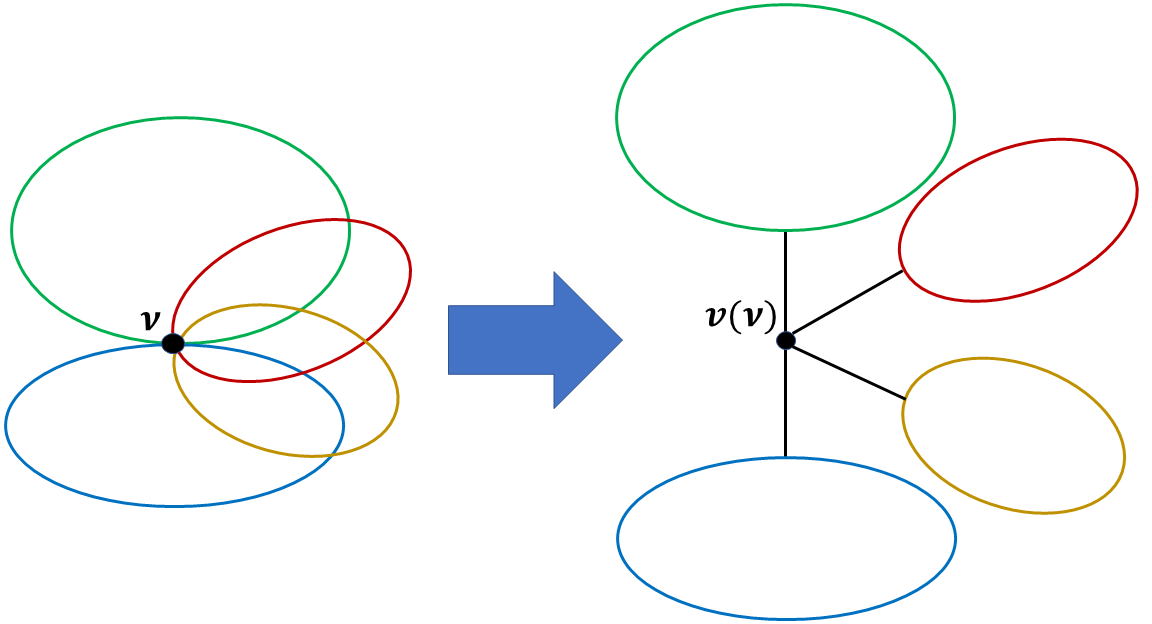
\includegraphics[width=0.6\textwidth]{src/images/Cactus-transformation.png}
    \caption{Transformation of cactus ${\cal H}_V$ to the tree $T({\cal H}_V)$.}
\label{fig:transform-cactus-to-tree}
\end{figure}

We know that if $\nu$ and $\mu$ are two nodes in the cactus, there exists a unique path of cycles and tree edges between them. It follows from the construction of $T({\cal H}_V)$ that the unique path between the vertices $v(\nu)$ and $v(\mu)$ captures the same path. Thus we state the following lemma.

\begin{lemma}
Let $\nu,\mu$ be any two arbitrary nodes in the cactus 
${\cal H}_V$. The unique path between $v(\nu)$ and $v(\mu)$ in $T({\cal H}_V)$ concisely captures all
paths between $\nu$ and $\mu$ in ${\cal H}_S$.
\label{lem:path-in-T(H_S)}
\end{lemma}

% Let $\nu$ and $\mu$ be any two nodes in skeleton ${\cal H}_S$. If they belong to the same cycle, say $c$, there are two paths between them on the cycle $c$ itself - their union forms the cycle itself. Using the fact that any two cycles in  ${\cal H}_S$ can have at most one common node, it can be seen that these are the only paths between $\nu$ and $\mu$. Using the same fact, if $\nu$ and $\mu$ belong to different cycles, there exists a unique sequence of alternating cycles and nodes $\langle \nu_1,c_1,\ldots,\nu_r,c_r,\nu_{r+1}\rangle $ satisfying the following 2 properties. \begin{itemize}
%     \item $\nu_1=\nu$, $\nu_{r+1}=\mu$, and for each $1< i\le r$, $\nu_i$ is the unique node common to $c_{i-1}$ and $c_i$.
%     \item Each path between $\nu$ and $\mu$ can be seen as a sequence $\langle p_1,\ldots p_r\rangle$ such that $p_i$ is a path between $\nu_i$ and $\nu_{i+1}$ on cycle $c_{i}$.
% \end{itemize}
% It follows from the construction of $T({\cal H}_S)$ that $\langle v(\nu_1),v(c_1),\ldots,v(\nu_r),v(c_r),v(\nu_{r+1})\rangle$ is the path between $v(\nu)$
% and $v(\mu)$. 
% Thus we can state the following lemma.
% \begin{lemma}
% Let $\nu,\mu$ be any two arbitrary nodes in the cactus 
% ${\cal H}_S$. The unique path between $v(\nu)$ and $v(\mu)$ in $T({\cal H}_S)$ concisely captures all
% paths between $\nu$ and $\mu$ in ${\cal H}_S$.
% \label{lem:path-in-T(H_S)}
% \end{lemma}

We root the tree $T({\cal H}_V)$ at any arbitrary vertex and augment it suitably so that it can answer any LCA query in $\mathcal O(1)$ time using \cite{DBLP:journals/jal/BenderFPSS05}. Henceforth, we shall use skeleton tree $T({\cal H}_S)$ to denote this data structure.

\section{Compact representation for all Steiner mincuts} \label{subsec:connectivity-carcass}

% Let $G=(V,E)$ be an undirected unweighted graph and $S\subseteq V$ be a subset (Steiner set) of its vertices. 
Dinitz and Vainshtein \cite{DBLP:conf/stoc/DinitzV94} designed a data structure $\mathfrak{C}_S = ({\cal F}_S,{\cal H}_S, \pi_S)$ that stores all the Steiner mincuts for a Steiner set $S\subseteq V$ in the graph. We present a summary of this data structure.

This data structure can be seen as a generalization of two already discussed data structures,
~(i) strip ${\cal D}_{s,t}$ storing all $(s,t)$-mincuts, and
~(ii) cactus graph ${\cal H}_V$ storing all global mincuts.

Two $S$-mincuts are said to be equivalent if they divide the Steiner set $S$ in the same way. The equivalence classes thus formed are known as the \textit{bunches}. Similarly, two vertices are said to be equivalent if they are not separated by any Steiner mincut. The equivalence classes thus formed are known as \textit{units}. A unit is called a \textit{Steiner unit} if it contains at least a Steiner vertex.

Let $(S_B,{\bar S_B})$ be the $2-$partition of Steiner set induced by a bunch $\cal B$. If we compress all vertices in $S_B$ to $s$ and all vertices in ${\bar S_B}$ to $t$, the strip ${\cal D}_{s,t}$ will store all cuts in ${\cal B}$. We shall denote this strip by ${\cal D}_{\cal B}$. Any such strip has the following property -- if two non-terminals nodes of two strips intersect at even one vertex then these nodes coincide and the inherent partitions of these nodes in both strips coincide as well.

The first component of the connectivity carcass is the \textit{flesh graph} ${\cal F}_S$ which is a generalization of the strip. This graph is a quotient graph of graph $G$. The vertices of ${\cal F}_S$ can be obtained by contracting each unit of $G$ to a single vertex. Thus, we denote the vertices of ${\cal F}_S$ simply by units. In addition to it, each unit of ${\cal F}_S$ is assigned a $2-$partition known as the \textit{inherent partition} on the set of edges incident on it. Any unit that appears as a non-terminal in the strip corresponding to some bunch is called a \textit{stretched unit}. Otherwise, it is called a \textit{terminal unit}. 
% Another distinction between these two units follows from the two observations made on strip corresponding to a bunch mentioned above. 
The inherent partition assigned to a stretched unit consists of two sets of equal cardinality. On the other hand, inherent partition assigned to a terminal unit is a trivial partition (one of the set is empty). Note that all Steiner units are terminal units but the reverse is not true.
% The concept of reachability is slightly modified in ${\cal F}_S$. Whenever we say that a unit $u$ is reachable from unit $u'$, it means that there exists a coherent path between $u$ and $u'$. A \textit{coherent path} refers to a sequence of units and edges in flesh $(u_1,e_1,u_2,e_2,\ldots,u_k)$ such that any $e_i$ is incident on $u_{i-1}$ and $u_i$ and for any $u_i$ $e_{i-1}$ and $e_i$ lie in different side of the inherent partition. The structure of the flesh graph implies that it is not possible for a coherent path to start and finish at a single unit and hence, ${\cal F}_S$ is in a sense acyclic. A \textit{transversal} refers to a $2-$partition of units such that any coherent path intersects it at most once. It can be shown that each transversal in the flesh ${\cal F}_S$ corresponds to a Steiner mincut.
The concept of reachability in ${\cal F}_S$ is similar to the strip. Whenever we say that a unit $u$ is reachable from unit $u'$, it means that there exists a coherent path between $u$ and $u'$. The structure of ${\cal F}_S$ is such that a coherent path cannot start and finish at a single unit and hence, ${\cal F}_S$ is in a sense acyclic. There is a one-to-one correspondence between transversals in ${\cal F}_S$ and Steiner mincuts in $G$.

The second component of the connectivity carcass, skeleton ${\cal H}_S$, is a cactus graph. 
To avoid confusion with the original graph, the vertices and edges of the skeleton will be referred to as nodes and structural edges respectively. 
% A structural edge in the skeleton is a tree-edge if it is not part of a cycle, otherwise, it is a cycle-edge. 
% If $c_S$ is the value of the Steiner mincut, then each tree-edge is assigned weight $c_S$ and each cycle-edge is assigned weight $\frac{c_S}{2}$. 
Each terminal unit of ${\cal F}_S$ is mapped to a node in the skeleton ${\cal H}_S$ by projection mapping ${\pi}_S$. A stretched unit on the other hand is mapped to a set of edges corresponding to a proper path in ${\cal H}_S$ by ${\pi}_S$. A \textit{proper path} in the skeleton refers to an alternating sequence of nodes and structural edges $(\nu_1,\epsilon_1,\nu_2,...,\nu_k)$ such that $\epsilon_i$ is incident on $\nu_{i-1}$ and $\nu_i$ and it intersects each cycle of the skeleton at at most one structural edge. 
% A \textit{subbunch} is a subset of a bunch that can be represented by a strip. 
All the bunches can be stored in a skeleton ${\cal H}_S$ in the form of subbunches (disjoint subsets of a bunch). Each cut in skeleton corresponds to a subbunch. The strip ${\cal D}_{\cal B}$ corresponding to this subbunch $\cal B$ can be obtained as follows. Let the cut in the skeleton separates it into two subcactuses ${\cal H}_S(\cal B)$ and ${\bar {\cal H}_S(\cal B)}$. If $P(\nu_1,\nu_2)$ be the path in the skeleton to which a unit $u$ is mapped, it will be placed in ${\cal D}_{\cal B}$ as follows.
\begin{itemize}
    \item If both $\nu_1$ and $\nu_2$ lie in ${\cal H}_S(\cal B)$ (or ${\bar {\cal H}_S(\cal B)}$) $u$ is contracted in source (or sink).
    \item Otherwise, $u$ is kept as a non-terminal unit.
\end{itemize}


Now we discuss an important property between the reachability of a stretched unit $u$ and the proper path to which it is mapped in the skeleton ${\cal H}_S$.

\begin{lemma}[\cite{DBLP:conf/soda/DinitzV95}]
Let $u$ be a stretched unit and $u'$ be any arbitrary unit in the flesh ${\cal F}_S$ and $\pi_S(u) = P(\nu_1,\nu_2)$, $\pi_S(u') = P(\nu_3,\nu_4)$. If $u'$ is reachable from $u$ in direction $\nu_2$, then both these paths are extendable to a larger proper path with $P(\nu_1,\nu_2)$ as the initial part and $P(\nu_3,\nu_4)$ as the final part.
\label{lem:path-extendable}
\end{lemma}

\begin{lemma}[\cite{DBLP:conf/stoc/DinitzV94}]
\label{lem:strip-from-carcass}
Let $s,t \in S$ such that $c_{s,t}=c_S$. Given the connectivity carcass ${\mathfrak C}_S$ storing all Steiner mincuts, the strip ${\cal D}_{s,t}$ can be constructed in time linear in the size of flesh graph.
\end{lemma}

The size of flesh ${\cal F}_S$ is ${\cal O}(\min(m,\tilde{n}c_S))$ where $\tilde{n}$ is the number of units in ${\cal F}_S$. The size taken by skeleton is linear in the number of Steiner units. Thus, overall space taken by the connectivity carcass is ${\cal O}(\min(m,\tilde{n}c_S))$.
%% \appendix
%% \include{appa}
%% \include{appb}
%% %% This defines the bibliography file (main.bib) and the bibliography style.
%% If you want to create a bibliography file by hand, change the contents of
%% this file to a `thebibliography' environment.  For more information 
%% see section 4.3 of the LaTeX manual.
% \begin{singlespace}
\bibliography{main}
\bibliographystyle{plain}
% \end{singlespace}

%% \end{document}

%% Comment: to include appendices use a single \appendix command followed 
%% by a number of \include{} commands as many files as needed, each of 
%% which should contain a \chapter{} command for the appendix title.
